% 1. Introduction
%    - What is MRI and why is it used clinically 
\gls{mri} or Magnetic Resonance Imaging is a medical imaging modality that uses magnetic fields and radiofrequency (\gls{rf}) energy, rather than ionizing radiation like X-rays, to produce images. These images are made by processing the signals produced when the net magnetization vector returns to equilibrium following an \gls{rf} excitation pulse. In fact, \gls{mri} has exceptional utility in clinical settings, particularly for neurological and musculoskeletal imaging, because it produces images with high sensitivity to anatomical variations and superior soft tissue contrast \cite{bushberg2011}. 

This contrast comes from the proton density and how freely their water molecules move within different tissue types such as fat, gray matter, white matter, and cerebral spinal fluid. When placed in a strong static magnetic field, these hydrogen-rich tissues develop a net equilibrium magnetization aligned with the field. An \gls{rf} pulse temporarily disturbs this equilibrium, and each tissue returns to it at a characteristic times of relaxation that define image contrast. Importantly, generating and sustaining this equilibrium magnetization, requires an exceptionally strong magnetic field.

% 2. Magnetic Interactions
% first about the field
To fully characterize the safety considerations relevant to epicardial leads, we must first understand the components of the system. An \gls{mri} scanner is constituted by five main components: the main magnet, the gradient coils, the \gls{rf} coils, the control electronics, and the console or computer for display \cite{Prince_MedicalImaging_2015}. A real example of this system can be found on Chapter \ref{ch:matsNmets}. 

Figure \ref{fig:scannerDesign} shows an exploded view of three cylindrical components arranged concentrically around what would be the patient couch at the center. These cylinders represent the primary magnetic field–generating structures, which must be isolated from the external environment. The outermost and largest cylinder corresponds to the main magnet, which houses superconducting windings capable of generating high magnetic field strength. The magnetic field strength, also known as magnetic flux density ($B$), is measured in Tesla (T). An alternative unit is the gauss (G), where 1 T = 10,000 G. For perspective, a clinical \gls{mri} scanner has a range from 0.5 T to 3 T, and up to 9 T in some systems of magnetic field strength, orders of magnitude stronger than Earth's magnetic field (0.5 G)\cite{bushberg2011, Prince_MedicalImaging_2015,lowrie1997fundamentals}. %Field uniformity is achieved through shimming while confinement is solved with proper shielding.

\begin{figure}[hbt!]
	\centering
	%\subfloat[%Diagram illustrating the main five components of an MRI scanner. 
		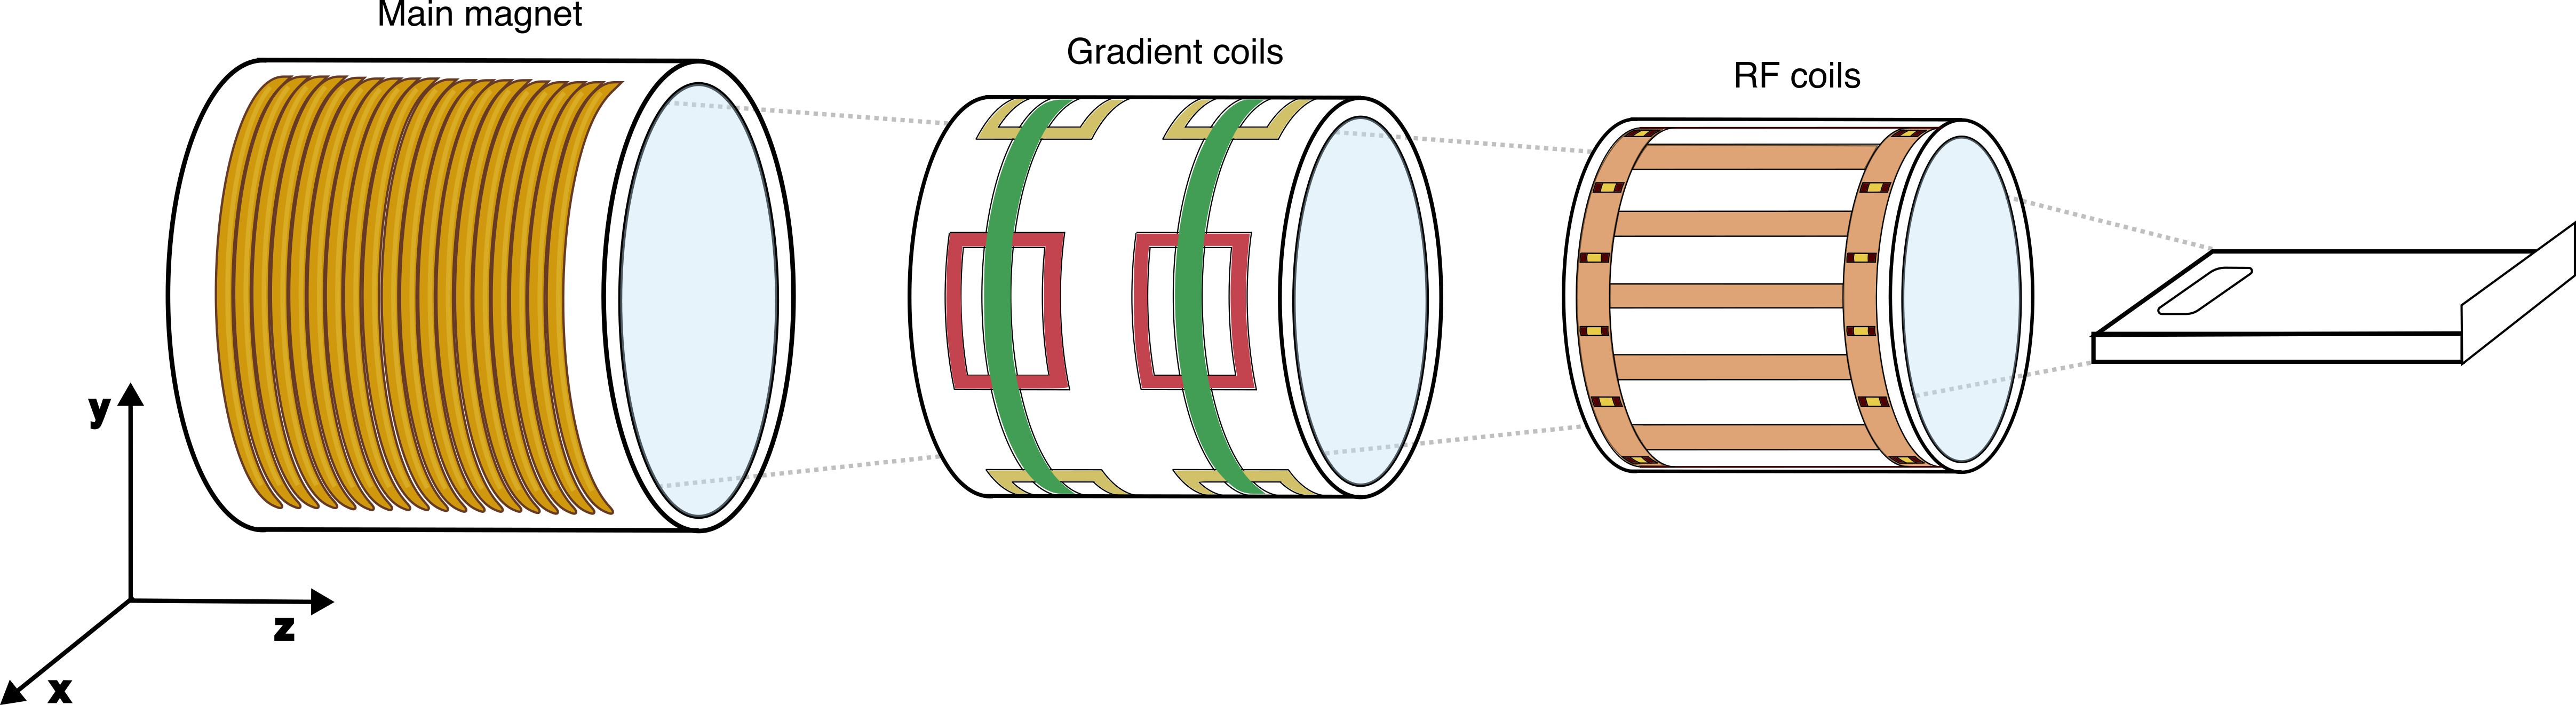
\includegraphics[width=0.90\textwidth]{Assets/mricomps.png}
	\caption[Design schematic of an MRI scanner]{The main components of an MRI scanner associated with safety hazards: the main magnet, gradient coils, and RF system.}
	\label{fig:scannerDesign}
\end{figure}

The magnetic field strength required for clinical imaging is sufficient to interact with materials normally considered non-magnetic in everyday context. The image formation exploits the microscopic magnetic behavior of atomic nuclei within this field. Hydrogen (specifically its proton, $^1H$) is the most utilized element in clinical \gls{mri} because it has the largest magnetic moment and is highly abundant in biological tissues, primarily in water and fat, which constitute the majority of soft tissue composition. 

Normally, these hydrogen atoms have a random orientation of their nuclear magnetic moments (protons) due to thermal energy. When placed in a strong static magnetic field ($B_0$), these nuclear magnetic moments weakly align in parallel (same direction of $B_0$, low-energy state) and antiparallel (opposite direction of $B_0$, high-energy state) directions. 

In addition to aligning with $B_0$, the protons also experience precession, much like the Earth’s rotation around its tilted axis or a spinning top under gravity. This precession occurs at an angular frequency ($\omega_0$) known as the Larmor frequency, which is directly proportional to the magnetic field strength ($B_0$), as described by the Larmor equation $\omega_0 = \gamma B_0.$ This frequency also corresponds to the separation between the proton’s magnetic energy levels, and it is the resonance condition in which an \gls{rf} pulse can be applied to make the transition between these states happen.

%RF coils role
In Figure \ref{fig:scannerDesign}, the innermost cylinder represents a birdcage resonator or body coil used to transmit \gls{rf} into the patient. Once this \gls{rf} pulse ($B_1$) is applied, synchronized to the Larmor frequency of protons (about 42.58 MHz per tesla), the protons excite and the net magnetization ($M$) tips away from the longitudinal direction ($z$) becoming anti-aligned. In doing so, it causes the magnetic moments of many protons to become synchronized, or phase-coherent. They start to precess together in the transverse plane, creating transverse magnetization ($M_{xy}$).

The instant the \gls{rf} pulse is turned off, the relaxation process starts, these precessing protons start to lose that synchronization due to slight variations in their local magnetic environments. This causes the transverse magnetization signal to gradually fade over time. The decaying oscillations of this signal are detected by the receiver coil, which potentially can be the same that sent them. The time at which the plane ($M_{xy}$) decays is described as transverse relaxation (T2). And the process in which the nuclear spins return to alignment along $B_0$ occurs with characteristic time T1 (longitudinal relaxation). The final \gls{mri} image's depiction of a tissue's brightness or darkness is determined by the \gls{rf} signal produced during these relaxation processes taken together.  

%gradient fields role
However, this covers one a single signal from a particular spot. Spatial localization of the signal requires knowing the origin of each measurement across all three axes. This is achieved using small, precisely controlled variations in the magnetic field known as gradient fields. The gradient fields are superimposed on $B_0$ and make the magnetic field slightly stronger or weaker depending on position, causing the Larmor frequency of the protons to vary with location.

In practice, three gradient coils systems work together to map space. Their configuration is depicted on Figure \ref{fig:scannerDesign} color-coded. First, a \gls{ssg} (green) selects, typically along the z-axis, a particular axial ``slice” of the body that is being excited by the \gls{rf} pulse. This defines the plane of imaging. Then, a \gls{peg} in yellow, briefly changes the precession speed of protons along an orthogonal axis, i.e. the y-axis, giving each row of tissue a unique phase ``signature". Finally, a \gls{feg} is applied along the x-axis, showed as red, so that protons precess at slightly different frequencies during signal readout. 

Each of these three subsystem is associated with distinct physical interactions that become relevant when conductive or magnetic objects, such as surgical hardware, are present in the scanner environment. For example, the static magnetic field spatial gradient exerts translational forces in the fringe field, rapid switching gradient is required to accomplish spatial encoding, but can induce peripheral nerve stimulation and acoustic noise, and RF coils deposit energy that may lead to tissue heating \cite{mriquestions_dangerous_place, mriquestions_gradient_safety, mriquestions_rf_safety}. These safety concerns are further explored in Section \ref{sec:concerns}.

Continuing on the image acquisition steps, the resulting signals are stored in a frequency domain matrix called k-space. Each line in k-space represents one measurement with a specific gradient configuration. When all necessary lines are filled, the Fourier Transform reconstructs the data into a spatial image, where each pixel corresponds to a small volume element (voxel) of tissue.

The control and computing subsystems coordinate every stage of image acquisition and reconstruction. The host computer and operator console provide the interface through which the technologist selects and supervises scanning protocols, while the pulse programming and measurement control systems synchronize gradient and RF activity \cite{bushberg2011}. Supporting units such as the digitizer, image processor, and compute engine translate the raw analog signals into interpretable digital images through Fourier-based reconstruction algorithms \cite{Prince_MedicalImaging_2015}. Finally, the dedicated power supplies, patient table mechanics, and electromagnetic shielding ensure stable operation, patient positioning, and noise minimization. Of these elements, the static field of the main magnet is the most significant to comprehend for this study as it establishes the imaging environment and is the major source of mechanical risk for implanted devices.
%static field effect
\subsection{Physics of the Static Field}
\label{sec:PhyField}
% 1. - Main Magnet                                   [🔴 High Priority]
%      (Primary source of static magnetic field and spatial gradients.)

Electric current flowing through a wire coil generates a magnetic field, and is the fundamental physical principle of the MR system. Field strength, temporal stability, and homogeneity are used to evaluate system performance. Clinical \gls{mri} main magnets are typically made of superconducting wire-wrapped cylinders. These wires are made from niobium-titanium alloys and show no resistance to electric current when maintained at extremely low temperatures and align the field along the patient's cranial-caudal axis \cite{Prince_MedicalImaging_2015}. 

The amplitude of the current $I$ and $n$, the turn density (turns per unit length), represent together the two quantities that determine the magnetic field strength magnitude for an ideal solenoid $B = \mu_{0} \, n I$. The field is directed along the solenoid's long axis. A good estimate of the magnetic field at position z along the bore axis, measured from the solenoid center,within a finite solenoid of length $L$ and radius $R$ can be calculated from Biot–Savart's law 

\begin{equation}
	B(z) = \frac{\mu_0 n I}{2} 
	\left[
	\frac{z + \frac{L}{2}}{\sqrt{R^2 + \left(z + \frac{L}{2}\right)^2}} 
	-
	\frac{z - \frac{L}{2}}{\sqrt{R^2 + \left(z - \frac{L}{2}\right)^2}}
	\right],
\end{equation}

\noindent where $\mu_0$ is the permeability of free space \cite{griffiths2013electrodynamics}. This formula provides the axial field along the solenoid, with the maximum occurring at the center ($z=0$) and decreasing smoothly toward the ends. A simulation of this model for a 1.4 $m$ length by 0.6 $m$ diameter ideal solenoid was used, to approximate a real \gls{mri} system, such as the Siemens Magnetom Trio\textsuperscript{\texttrademark}, used at \gls{bergan}.

Figure \ref{fig:Bz_vs_zSet} showcases this model in two parts. First, the magnetic field ($B_0$) along the z-axis, where $z=0$ corresponds to isocenter with dashed vertical lines and light blue shading marking the solenoid boundaries at z = $\pm$ 0.704 m away from isocenter. The field is normalized to a maximum of $B_0 = 3$~T, shown as a dashed horizontal reference line, with no shielding or distortion applied. 

\begin{figure}[htb!]
	\centering
	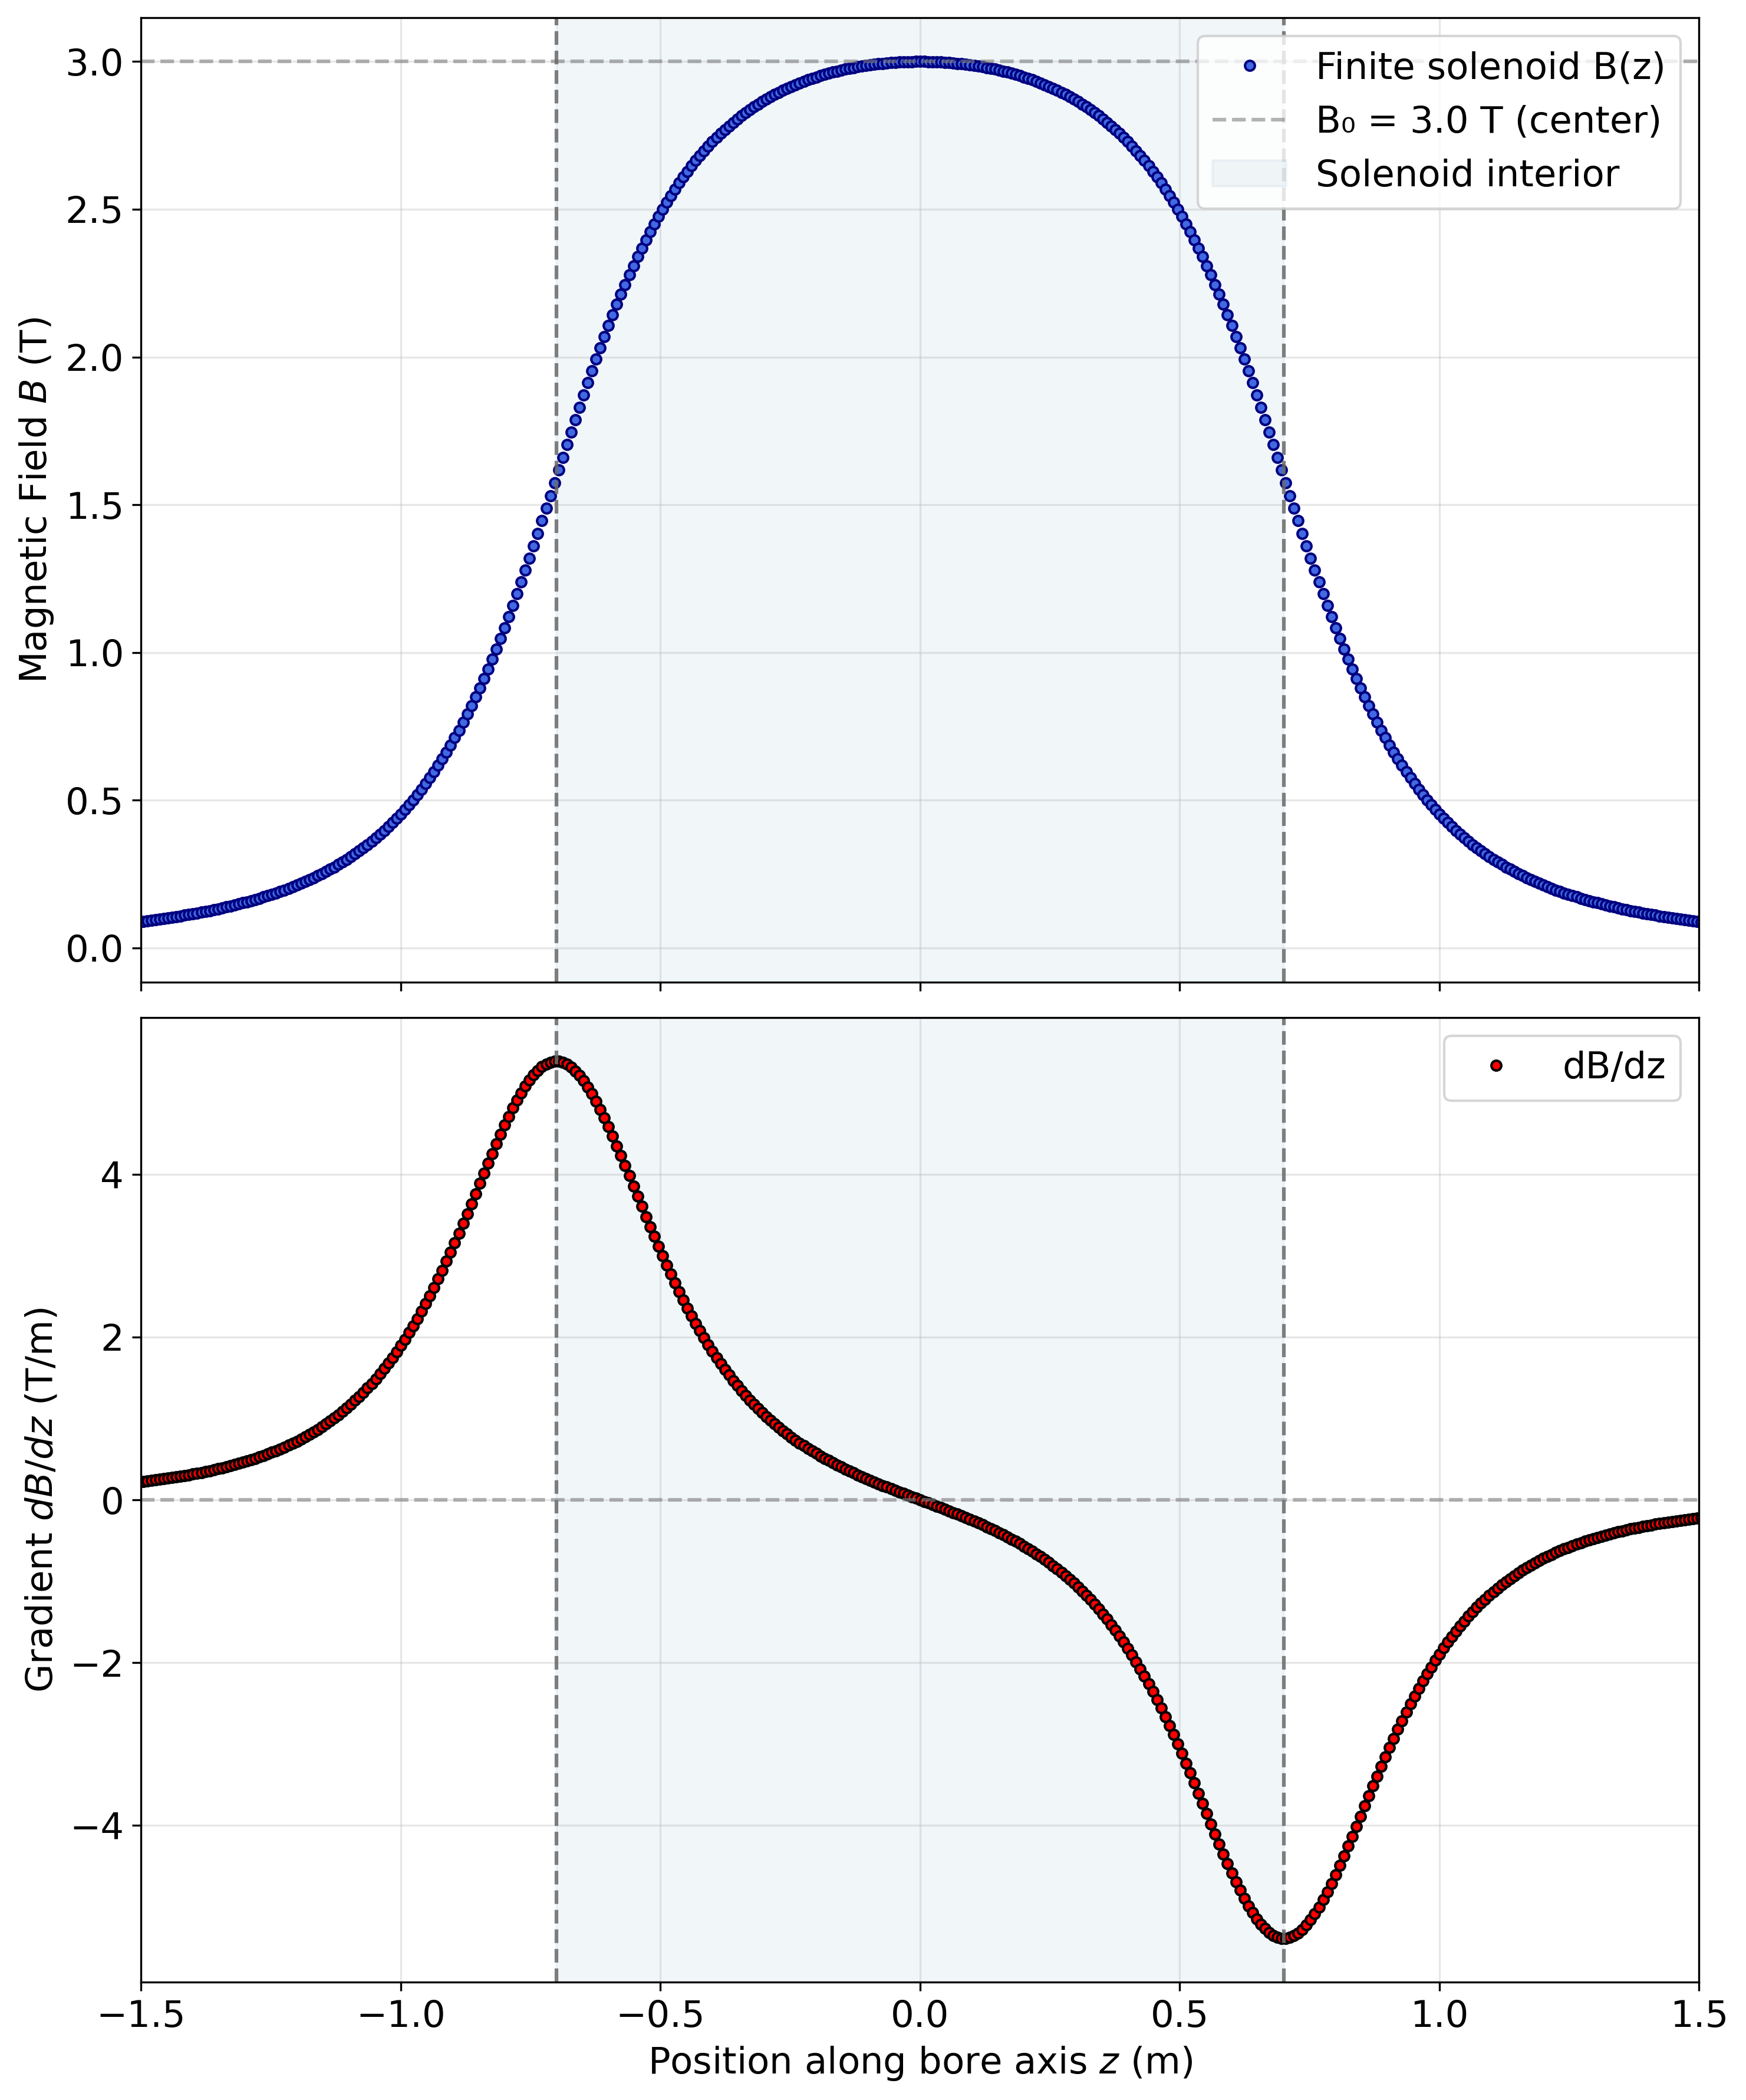
\includegraphics[width=0.65	\textwidth]{Assets/FieldMapping.png}
	\caption[Axial magnetic flux density $B_z$ and spatial gradient for an idealized 3 T MRI solenoid]{Axial magnetic flux density $B_z$ and spatial gradient for an idealized 3 T \gls{mri} solenoid (L = 1.4 $m$, R = 0.3 $m$). Top: The magnetic field peaks at 3T at the isocenter (z = 0 $m$) and decreases symmetrically toward both ends. Grey dotted lines indicate the solenoid edges (bore entrances). Bottom: The spatial gradient $dB_z/dz$ reaches its maximum magnitude at the bore entrances (z = ±0.704 $m$).}
	\label{fig:Bz_vs_zSet}
\end{figure}

Second, the axial field $B(z)$ from the finite solenoid model yields a spatial gradient $dB_z/dz$, its maximum value is confirmed to be at the bore entrance position \cite{astmF2052,ferreira2017} ($z \approx \pm 0.704$ m for this 1.4 m length example), as shown in the bottom panel of Figure \ref{fig:Bz_vs_zSet}. These strong gradients (often several T/m near entrances) exert attractive forces on paramagnetic/ferromagnetic objects (pulling toward higher $|B|$) and repulsive on diamagnetic ones (pushing away), posing projectile hazards \cite{bushberg2011,astmF2052,ferreira2017}. This gradient-driven behavior supports ASTM displacement force testing and motivates shielding designs in modern systems. High-susceptibility materials experience the strongest pull toward the isocenter, with the maximum risk at bore entrances.

Having established the spatial distribution of the static field, we now turn to how this field interacts with matter. These interactions are governed by fundamental electromagnetic theory and provide the foundation for classifying materials by magnetic susceptibility which quantifies \gls{mri} safety risks for implanted devices according to ASTM standards \cite{astmF2052,astm2213}.

\subsection{The Static Field interaction with matter}

Any material placed in a magnetic field develops a magnetization, $\mathbf{M}$, defined as the net magnetic dipole moment per unit volume, $\mathbf{M} \equiv \frac{\boldsymbol{m}}{V}$ \cite{griffiths2013electrodynamics}. In a way this  $\mathbf{M}$ represents a ``smoothed'' magnetization of an average field effect over many atoms. At the atomic level, the magnetic field inside a material fluctuates rapidly due to particles in motion. This phenomena forms the basis for \gls{mri} image generation. However, for the purpose of this thesis, we focus on the macroscopic behavior mostly. To simplify the macroscopic analysis of materials in magnetic fields, the auxiliary magnetic field $\mathbf{H} \equiv \frac{1}{\mu_0} \mathbf{B} - \mathbf{M}$, where $\mathbf{B}$ is the macroscopic magnetic flux density and $\mu_0$ is the permeability of free space, accounts for the contribution to the magnetic field from free currents, separating it from the contribution of bound currents induced by magnetization \cite{griffiths2013electrodynamics}. This distinction becomes useful when analyzing mechanical effects on magnetic dipoles.

Different materials respond differently to an applied field. For linear materials magnetization is also directly proportional to the field strength $\mathbf{M} = \chi_m \mathbf{H}$, the degree to which a material becomes magnetized is quantified by its magnetic susceptibility, $\chi_m$, which is typically around $-10^{-5}$ to 0 for biological tissues. It is convenient to define the material permeability as $\mu \equiv \mu_0(1 + \chi_m)$, so that the magnetic flux density takes the compact form

\begin{subequations}
	\begin{align}
		\mathbf{B} &= \mu_0(1+\chi_m)\mathbf{H} \quad \text{or} \label{eq:B_linear} \\
		\mathbf{B} &\approx \mu\mathbf{H} \label{eq:B_approx}
	\end{align}
\end{subequations}

Diamagnetic materials, such as water, calcium, and most organic compounds, develop a magnetization opposite to the applied B-field due to paired electrons. The susceptibilities of most human tissues are very small, in the range from -7$\times10^{-6}$ to -11.0$\times10^{-6}$. Paramagnetic substances, like molecular oxygen, deoxyhemoglobin, or gadolinium-based \gls{mri} contrast agents, align weakly with the field, enhancing the local magnetic flux with $\chi_m$ values from 0 to $+10^{-2}$ \cite{Schenck2000}. Contrast agents, such as gadolinium or iron‑oxide, represent a separate class of regulated pharmaceuticals administered only in carefully controlled doses \cite{Shah2023}. 

For this material types, relevant to MR environment, the susceptibility satisfies ($|\chi_m| \ll 1$), and Eq. \ref{eq:B_approx} reduces to $B = \mu_0 H$. Ferromagnetic materials, by contrast, exhibit strong self-sustained magnetization, about $10^2$ to $10^5$, and are avoided in \gls{mri} suites due to safety hazards \cite{Stafford2020}. This classification directly determine how the components of an implanted device such as an epicardial pacing lead respond mechanically to the \gls{mri} static field, which is the primary topic of this work.

%Figure \ref{fig:chi_spectrum} shows a spectrum of magnetic susceptibilities highlighting the region \gls{mri} where water and most human tissue is found.

%\begin{figure}[htb!]
%\centering
%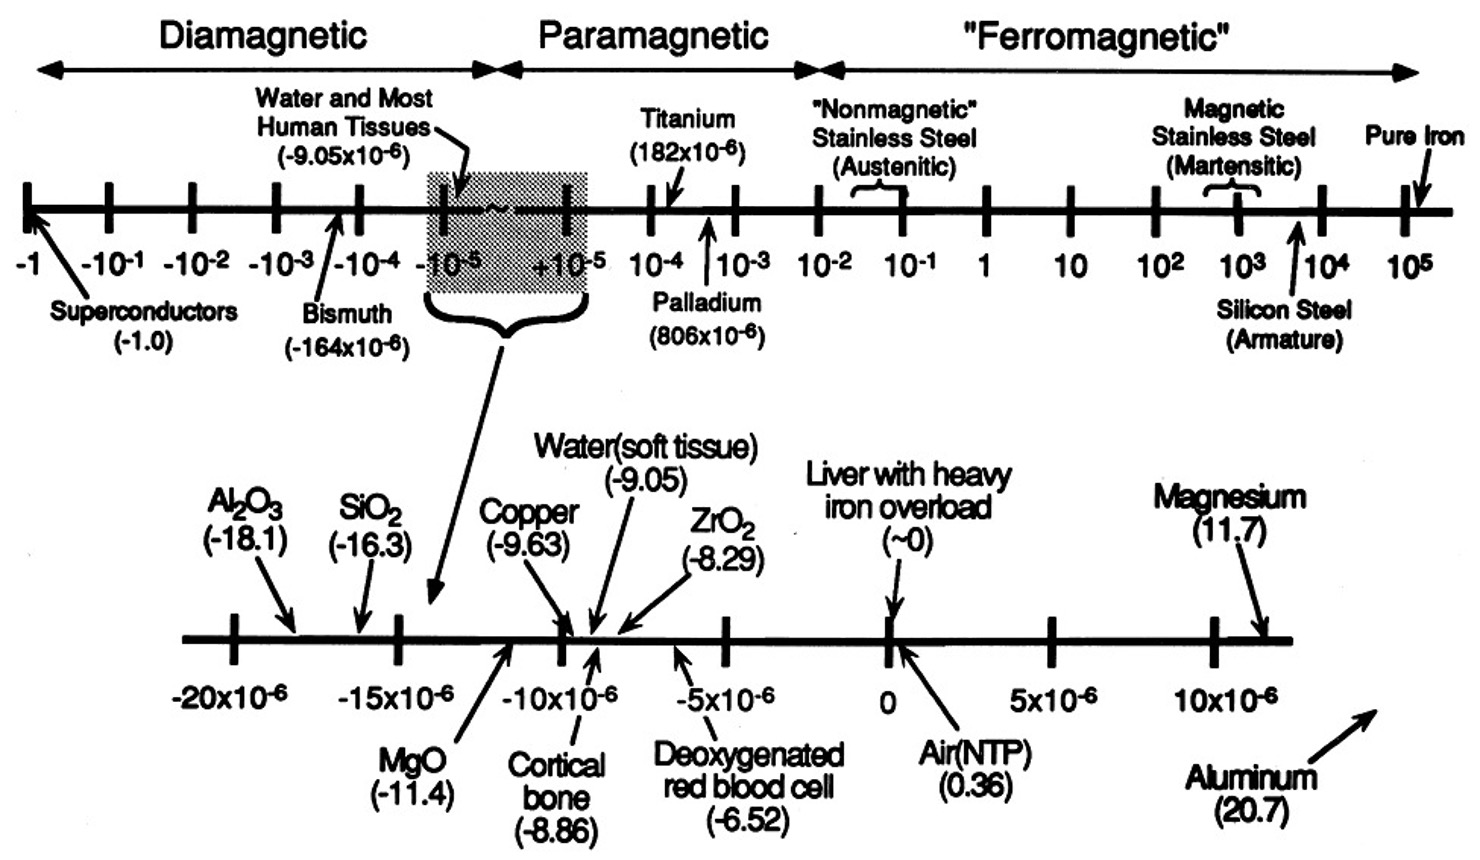
\includegraphics[width=0.95\textwidth]{Assets/Chi_inMRI.jpg}
%\caption[Spectrum of magnetic susceptibilities.]{
	%Spectrum of magnetic susceptibilities. The upper diagram uses a logarithmic scale to indicate the full range of observed magnetic susceptibility values, extending from -1.0 for superconductors to 100,000 for soft ferromagnetic materials. The bottom diagram uses a linear scale (in ppm) to indicate the properties of some materials with 20 ppm. The susceptibilities of most human tissues are in the range from -7.0 to -11.0 ppm. Adapted from Schenck \cite{Schenck2000}.}
%\label{fig:chi_spectrum}
%\end{figure}

%\subsection{Image generation}
%\label{sec:imageGen}
%% ------------------------------------------------------------------------------
% MRI Translational Forces – Background Section Writing Guide
%
% Section Structure with Topic Priorities:
%
% 1. Introduction
%    - What is MRI and why is it used clinically      [🟠 Medium Priority]
%      (Keep brief—serves as justification for MRI relevance to clinical care.)
%
% 2. Magnetic Interactions
%    - Magnetic Moments & Magnetization              [🔴 High Priority]
%      (Foundation for understanding how magnetic fields act on materials.)
%    - Material Susceptibility (Δχ)                  [🔴 High Priority]
%      (Include MR compatibility thresholds—Δχ < 0.01 for safety.)
%
% 3. MRI System Components
%    - Main Magnet                                   [🔴 High Priority]
%      (Primary source of static magnetic field and spatial gradients.)
%    - Gradient Coils                                [🟠 Medium Priority]
%      (Include brief note on eddy currents and induced Lorentz forces.)
%    - RF Coils (Antennas)                           [🟡 Low Priority]
%      (Mention briefly if relevant to antenna effect in retained leads.)
%
% 4. Background Physics
%    - Resonance & Larmor Frequency                  [🟠 Medium Priority]
%      (Describe precession, gyromagnetic ratio; sets up how B₀ interacts with protons.)
%    - T1/T2 Relaxation                              [🟡 Low Priority]
%      (Tissue-level effects, not directly tied to mechanical forces; keep concise.)
%
% 5. Out of Scope (Omit or Defer to Appendix)
%    - Signal Localization and K-Space               [⚪ Skip]
%    - Image Acquisition Parameters & Weighting      [⚪ Skip]
%    - Basic Pulse Sequences                         [⚪ Skip]
%
% Legend:
%   🔴 High Priority   – Discuss in full detail
%   🟠 Medium Priority – Cover briefly, emphasize relevance
%   🟡 Low Priority    – One or two sentences max
%   ⚪ Skip            – Omit unless contextually needed
% ------------------------------------------------------------------------------

%from macroscopic to micro to continue image formation
While macroscopic magnetization ($M$) and susceptibility ($\chi_m$) govern bulk mechanical interactions and safety risks for implants, the diagnostic power of \gls{mri} arises from the microscopic magnetic properties of atomic nuclei. Hydrogen (specifically its proton, $^1H$) is the most utilized element in clinical MRI because it has the largest magnetic moment and is highly abundant in biological tissues, primarily in water and fat, which constitute the majority of soft tissue composition. In fact, \gls{mri} was originally named Nuclear Magnetic Resonance (NMR), because it involves the spectroscopic study of the magnetic properties of the atomic nucleus as it resonates and aligns with applied magnetic field changes. On the scale of elementary particles, these interactions involve the nuclear spin and charge distribution of protons and neutrons within the atomic nucleus. 

Normally, these hydrogen atoms have a random orientation of their nuclear magnetic moments (protons) due to thermal energy. When placed in a strong static magnetic field ($B_0$), these nuclear magnetic moments align in parallel (same direction of $B_0$, low-energy state) and antiparallel (opposite direction of $B_0$, high-energy state) directions. 

%This is illustrated in Figure~\ref{fig:proton_alignment}, notice that the distribution of protons into these two states is influenced by thermal energy and a slight majority align in the low-energy, parallel direction, resulting in an observable net magnetic moment (red arrow) usually denoted as equilibrium magnetization ($M_0$).

\begin{figure}[htb!]
	\centering
	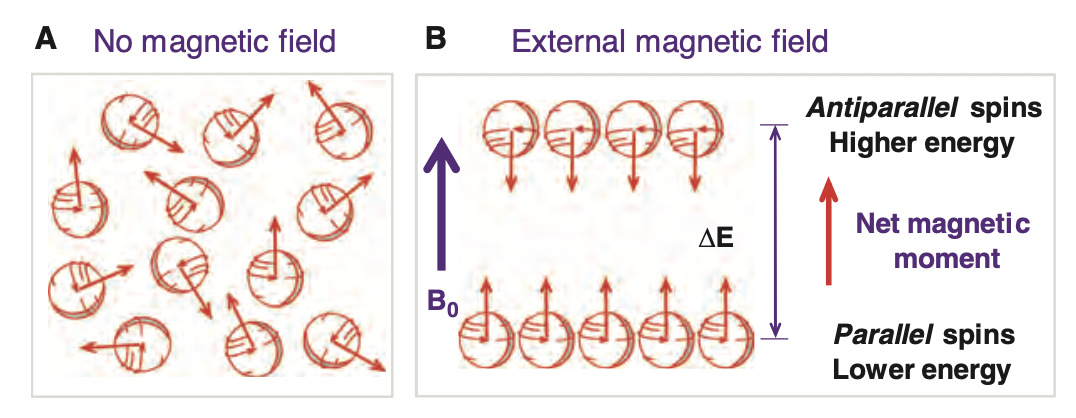
\includegraphics[width=\textwidth]{Assets/MRIproton.png}
	\caption[Proton alignment in a magnetic field]{Schematic illustration of how hydrogen protons ($^1$H) behave in the presence of a strong static magnetic field ($B_0$). 
		A: In the absence of a field, proton magnetic moments are randomly oriented, producing no net magnetization. 
		B: When exposed to $B_0$, protons align either parallel or antiparallel to the field. 
		From Bushberg, J.T., \textit{The Essential Physics of Medical Imaging} (2011) \cite{bushberg2011}.}
	\label{fig:proton_alignment}
\end{figure}


Depicted in Figure \ref{fig:protonPrecession}, the motion happens around the axis of the applied magnetic field due to the perpendicular torque they experience. 

\begin{figure}[htb!]
	\centering
	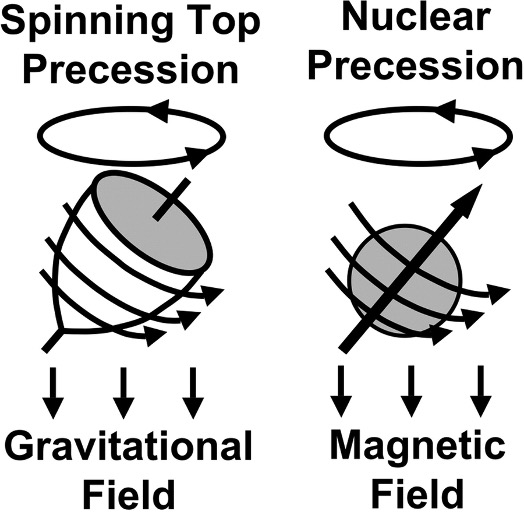
\includegraphics[width=0.55\linewidth]{Assets/protonPrecession.jpg}
	\caption[Analogy between proton spin precession and precession of a spinning top.]{Illustration of proton precession under a static magnetic field $B_0$ compared to that of a spinning top under gravity. Adapted from Pooley, R. A., \textit{Fundamental physics of MR imaging}, (2005) \cite{Pooley2005}.}
	\label{fig:protonPrecession}
\end{figure}

%Precession and Larmor frequency
In addition to aligning with $B_0$, the protons also experience precession, much like the Earth’s rotation around its tilted axis or a spinning top under gravity. This precession occurs at an angular frequency ($\omega_0$) known as the Larmor frequency, which is directly proportional to the magnetic field strength ($B_0$), as described by the Larmor equation $\omega_0 = \gamma B_0.$

%RF coils role
An \gls{rf} energy pulse ($B_1$) is then applied, synchronized to the Larmor frequency of protons (about 42.58 MHz per tesla), magnetizing the protons and tipping the net magnetization ($M$) away from the longitudinal direction ($M_z$). This pulse provides just enough energy for some protons to move into a higher energy state, also called RF excitation. In doing so, it also causes the magnetic moments of many protons to become synchronized, or phase-coherent. They start to precess together in the transverse plane, creating what is called transverse magnetization ($M_{xy}$).

The instant the RF pulse is turned off, the relaxation process starts, these precessing protons start to lose that synchronization due to slight variations in their local magnetic environments. This causes the transverse magnetization signal to gradually fade over time. The oscillations of this signal are detected by the same RF coils that sent them. %The strength and rate of decay of this signal are dependent on the tissue type and are characterized by two time constants: $T1$ and $T2$.

First, the signal in the transverse plane, ($M_{xy}$), decreases as the protons desynchronize, this is described by $T2$ (Transverse Relaxation). And the process by which the system regains equilibrium is described by $T1$ (Longitudinal Relaxation).  The longitudinal magnetization ($M_z$) returns, and the particles realign with the main magnetic field ($B_0$). The final \gls{mri} image's depiction of a tissue's brightness or darkness is determined by the RF signal produced during relaxation processes taken together.  %For instance, on $T1$-weighted images, tissues with short $T1$ times (such as fat) seem bright, whereas on $T2$-weighted images, tissues with longer $T2$ periods (such as cerebrospinal fluid) appear bright, see Figure~\ref{fig:T2vsT1}.

%\begin{figure}[htb!]
	%\centering
	%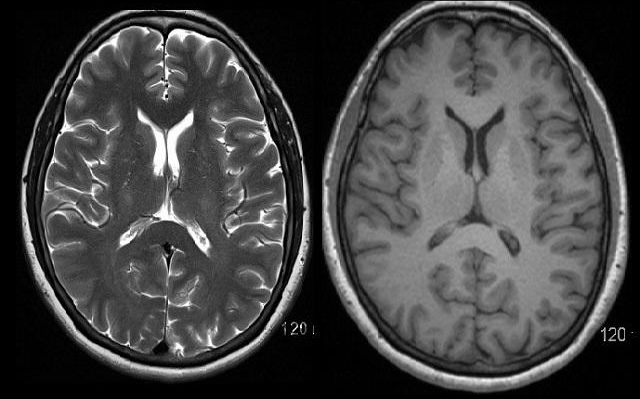
\includegraphics[width=0.65\textwidth]{Assets/T2vsT1.jpg}
	%\caption[Comparison between T1- and T2-weighted brain MRI images.]{Comparison between T1- and T2-weighted brain MRI images of the same subject. The left image shows a T2-weighted scan, where cerebrospinal fluid (CSF) appears bright, and the right image shows a T1-weighted scan, where fat and white matter appear bright. Adapted from \cite{riteadvantageT1T2}.}
	%\label{fig:T2vsT1}
%\end{figure}

%gradient fields role
However, this covers one a single signal from a particular spot. To make an image rather, the \gls{mri} system must know where each signal is coming from. This is achieved using small, precisely controlled variations in the magnetic field known as gradient fields. These gradient coils, superimposed on $B_0$, make the magnetic field slightly stronger or weaker depending on position, causing the Larmor frequency of the protons to vary with location.

Three gradient systems work together to map space. First, \gls{ssg} is a applied during excitation so that only protons in a particular “slice” of the body resonate at the RF pulse frequency. This defines the plane of imaging. Then, \gls{peg}, briefly changes the precession speed of protons in one direction, giving each row of tissue a unique phase ``signature". Finally, \gls{feg} is applied during signal readout so that protons along another axis precess at slightly different frequencies.

%\subsection{Scanner Design and Subsystems}

%As mentioned above, after the main static field ($B_0$) has been established and shimmed to high homogeneity the gradient coils introduce controlled spatial variation in the magnetic field for encoding localizing signals generated during MR. Gradient coils, are wire conductors located within the main bore of the magnet with typical strength values from 1 to 50 mT/m and correspond to the logical coordinate axes: x, y, and z which relate to \gls{ssg}, \gls{peg}, and \gls{feg}. They operate by adding to or subtracting from the magnitude of the main field ($B_0$), but they do not change the direction of the magnetic field \cite{bushberg2011}.

These gradients must switch rapidly and with large current flows, typical slew rate ranges from 5 to 250 mT/m/ms, with currents on the order of 100–200 A \cite{bushberg2011,Prince_MedicalImaging_2015}, to accomplish encoding. The resulting signals are stored in a matrix called k-space. Each line in k-space represents one measurement with a specific gradient configuration. When all necessary lines are filled, the Fourier Transform reconstructs the data into an image, where each pixel corresponds to a small volume element (voxel) of tissue.

The control and computing subsystems coordinate every stage of image acquisition and reconstruction. The host computer and operator console provide the interface through which the technologist selects and supervises scanning protocols, while the pulse programming and measurement control systems synchronize gradient and RF activity \cite{bushberg2011}. Supporting units such as the digitizer, image processor, and compute engine translate the raw analog signals into interpretable digital images through Fourier-based reconstruction algorithms \cite{Prince_MedicalImaging_2015}; Finally, the dedicated power supplies, patient table mechanics, and electromagnetic shielding ensure stable operation, patient positioning, and noise minimization. 

These same magnetic field components pose hazards can pose hazards to implanted conductive objects. Although most modern \gls{mri} systems are designed for patient safety, implanted devices and retained surgical materials introduce additional considerations. One clinically relevant example is epicardial leads, which are commonly placed during cardiac surgery to provide temporary postoperative pacing for arrhythmias. These leads consist of conductive wires (often stainless steel or similar alloys) sutured directly to the epicardial surface of the heart and may be removed postoperatively or, in some cases, cut short and abandoned in situ to avoid extraction risks.